% Этот шаблон документа разработан в 2014 году
% Данилом Фёдоровых (danil@fedorovykh.ru) 
% для использования в курсе 
% <<Документы и презентации в \LaTeX>>, записанном НИУ ВШЭ
% для Coursera.org: http://coursera.org/course/latex .
% Исходная версия шаблона --- 
% https://www.writelatex.com/coursera/latex/3.2

\documentclass[a4paper, 12pt]{article}

%%% Работа с русским языком
\usepackage{cmap}					% поиск в PDF
\usepackage{mathtext} 				% русские буквы в формулах
\usepackage[T2A]{fontenc}			% кодировка
\usepackage[utf8]{inputenc}			% кодировка исходного текста
\usepackage[english,russian]{babel}	% локализация и переносы

%%% Дополнительная работа с математикой
\usepackage{amsmath,amsfonts,amssymb,amsthm,mathtools} % AMS
\usepackage{icomma} % "Умная" запятая: $0,2$ --- число, $0, 2$ --- перечисление

%% Номера формул
%\mathtoolsset{showonlyrefs=true} % Показывать номера только у тех формул, на которые есть \eqref{} в тексте.
%\usepackage{leqno} % Нумерация формул слева

%% Свои команды
\DeclareMathOperator{\sgn}{\mathop{sgn}}

%% Перенос знаков в формулах (по Львовскому)
\newcommand*{\hm}[1]{#1\nobreak\discretionary{}
{\hbox{$\mathsurround=0pt #1$}}{}}

%%% Работа с картинками
\usepackage{graphicx}  % Для вставки рисунков
\graphicspath{{Materials/}{images2/}}  % папки с картинками
\setlength\fboxsep{3pt} % Отступ рамки \fbox{} от рисунка
\setlength\fboxrule{1pt} % Толщина линий рамки \fbox{}
\usepackage{wrapfig} % Обтекание рисунков текстом

%%% Работа с таблицами
\usepackage{array,tabularx,tabulary,booktabs} % Дополнительная работа с таблицами
\usepackage{longtable}  % Длинные таблицы
\usepackage{multirow} % Слияние строк в таблице

%%% Теоремы
\theoremstyle{plain} % Это стиль по умолчанию, его можно не переопределять.
\newtheorem{theorem}{Теорема}[section]
\newtheorem{proposition}[theorem]{Утверждение}
 
\theoremstyle{definition} % "Определение"
\newtheorem{corollary}{Следствие}[theorem]
\newtheorem{problem}{Задача}[section]
 
\theoremstyle{remark} % "Примечание"
\newtheorem*{nonum}{Решение}

%%% Программирование
\usepackage{etoolbox} % логические операторы

%%% Страница
%\usepackage{extsizes} % Возможность сделать 14-й шрифт
\usepackage{geometry} % Простой способ задавать поля
	\geometry{top=25mm}
	\geometry{bottom=25mm}
	\geometry{left=20mm}
	\geometry{right=20mm}
 %
\usepackage{fancyhdr} % Колонтитулы
 	\pagestyle{fancy}
 	\renewcommand{\headrulewidth}{0mm}  % Толщина линейки, отчеркивающей верхний колонтитул
 	\lfoot{}
 	\rfoot{}
 	\rhead{Верхний правый}
 	\chead{}
 	\lhead{ }
 	% \cfoot{Нижний в центре} % По умолчанию здесь номер страницы

\usepackage{setspace} % Интерлиньяж
%\onehalfspacing % Интерлиньяж 1.5
%\doublespacing % Интерлиньяж 2
%\singlespacing % Интерлиньяж 1

\usepackage{lastpage} % Узнать, сколько всего страниц в документе.

\usepackage{soulutf8} % Модификаторы начертания

\usepackage{hyperref}
\usepackage[usenames,dvipsnames,svgnames,table,rgb]{xcolor}
\hypersetup{				% Гиперссылки
    unicode=true,           % русские буквы в раздела PDF
    pdftitle={Заголовок},   % Заголовок
    pdfauthor={Автор},      % Автор
    pdfsubject={Тема},      % Тема
    pdfcreator={Создатель}, % Создатель
    pdfproducer={Производитель}, % Производитель
    pdfkeywords={keyword1} {key2} {key3}, % Ключевые слова
    colorlinks=true,       	% false: ссылки в рамках; true: цветные ссылки
    linkcolor=red,          % внутренние ссылки
    citecolor=green,        % на библиографию
    filecolor=magenta,      % на файлы
    urlcolor=cyan           % на URL
}

%\renewcommand{\familydefault}{\sfdefault} % Начертание шрифта

\usepackage{multicol} % Несколько колонок

% Мои "дополнительные" пакеты
\usepackage{textcase} 
\usepackage{pdfpages}
\usepackage{amsmath}


\author{Подкидышев Алексей}
\title{Студент МФТИ ФИВТ - 1ый курс}
\date{\today}

\begin{document} % конец преамбулы, начало документа

\thispagestyle{empty}
\begin{center}
	\textit{\MakeTextUppercase{федеральное государственное автономное учреждение}}
		
	\vspace{0.5ex}
	
	\textbf{ \\ \MakeTextUppercase{<<Московский Физико-технический институт>>}}
\end{center}
\vspace{13ex}
\begin{flushright}
	\noindent
	{Подкидышев Алексей Сергеевич}
	\\
	\textit{Студент факультета инноваций\\ и высоких технологий\\(группа 790)}
\end{flushright}
\begin{center}
	\vspace{23ex}
	\begin{LARGE}
	
	\textbf{Лабораторная работа №2.4.1}	

	\end{LARGE}	
	\vspace{1ex}
		
	\begin{large}
	
	\textbf
	
	\end{large}
	
	\vfill
	Долгопрудный 
	
	{\today}
\end{center}

\newpage

\section{Установка. Теоретический материал:}
\subsection{Оборудование}
\large
\textbf{В работе используются:} термостат; герметичный сосуд, заполненный исследуемой жидкостью; отсчетный микроскоп\\[3ex]

\rhead{Подготовка}

\begin{wrapfigure}[18]{l}{0.5\linewidth}\label{scheme}
	
	\includegraphics[scale=0.5]{scheme.png}
	\caption{Схема установки для определения теплоты испарения}
\end{wrapfigure}

Наполненный водой резервуар 1 играет роль термостата. Нагревание производится спиралью 2. Для охлаждения через змеевик 3 подается холодная вода. Вода в термостате перемешивается воздухом, поступающим через трубку 4. Температура воды измеряется термометром 5. В термостат погружен прибор 6 с исследуемой жидкостью (в нашем случае -- спирт). Над ней находится насыщенный пар. Давление пара определяется ртутным манометром, соединенным с исследуемым объемом. Отсчет показаний манометра производится с помощью микроскопа.\\[2ex]

\subsection{Описание/Цель работы}

\textbf{Цель работы:} Измерение давления насыщенного пара жидкости при различных температурах; 2) вычисление по полученным данным теплоты испарения с помощью уравнения Клапейрона-Клаузиуса.

\textit{Испарение} -- переход вещества из жидкого состояния в газообразное. Оно происходит со всей поверхности жидкости. Для испарения молекулы должны преодолеть силу молекулярного сцепления и совершить работу против внешнего давления $P$, поэтому не все молекулы способны совершить эту работу, а только те, которые обладают достаточной кинетической энергией. Поэтому переход части молекул в пар приводит к обеднению жидкости быстрыми молекулами, т.е. к ее охлаждению.

Количество теплоты, необходимое для изотермического испарения одного моля жидкости при внешнем давлении, равном упругости ее насыщенных паров, называется \textit{молярной теплотой испарения (парообразования)}. В настоящей работе используется метод определения теплоты испарения, основанный на уравнении Клапейрона-Клаузиуса:
\begin{equation}
\dfrac{dP}{dT} = \dfrac{L}{V_{2} - V_{1}}
\end{equation}
Здесь $P$ -- давление насыщенного пара при температуре $T$, $L$ -- теплота испарения жидкости, $V_1$ -- объем жидкости, $V_2$ -- объем пара. При нашей точности опытов величиной $V_1$ можно пренебречь (она составляет порядка 0,5\% объема пара). Обозначим $V_2 = V$. Объем связан с давлением и температурой уравнением Ван-Дер-Ваальса:
\begin{equation}
(P + \frac{a}{V^2})(V - b) = RT
\end{equation}
Однако в наших условиях пренебрежение константами $a$ и $b$ вносит погрешность менее 3\% при атмосферном давлении, а при более низких давлениях погрешность становится еще меньше. Положим
\begin{equation}
V = \dfrac{RT}{P}
\end{equation} 
Подставляя (3) в (1) и пренебрегая $V_1$, получим
\begin{equation}
L = \frac{RT^2}{P}\frac{dP}{dT} = -R\frac{d(\ln P)}{d(1/T)}
\end{equation}
\newpage
\section{Ход работы:}
\rhead{Ход работы}
\begin{enumerate}
\item
Измерим высоту слоя конденсата.\\	
Заметим, что над поверхностью ртути находится небольшой слой воды высотой $\Delta h = 9,2$ сm. Этот слой будет создавать добавочное давление $\Delta p = \rho g \Delta h \approx  90,16$ Па. Будем учитывать это давление при дальнейших подсчетах.
\item
Включим термостат. Будем достаточно медленно (чтобы температура спирта оставалось близкой к температуре воды) нагревать воду в калориеметре от температуры $T_0$ до $40^o$С. При этом с повышением температуры на 1 градус измеряем разность уровней в манометре. Перенесем данные в таблицу 1 (при измерении давления необходимо учесть поправку $\Delta p$). 

% Место для таблицы 1
\begin{table}[h]

\begin{center}
\label{my-label}
\begin{tabular}{|l|l|l|l|l|l|}
\hline
\textbf{$h_1, $cm} &\textbf{$h_2, $cm} & \textbf{$T, C^{\circ}$} & \textbf{T, K}  & \textbf{$\vartriangle H, m$} & \textbf{$P, 10^3 $ Па} \\ \hline
10,15  & 5,53   & 20,27        & 293,4 & 0,046       & 6,049                      \\
10,53  & 5,27   & 22           & 295,2 & 0,053       & 6,900                      \\
10,83  & 4,89   & 24           & 297,2 & 0,059       & 7,803                      \\
11,12  & 4,58   & 26           & 299,2 & 0,065       & 8,601                      \\
11,45  & 4,2    & 28           & 301,2 & 0,073       & 9,544                      \\
11,8   & 3,75   & 30           & 303,2 & 0,081       & 10,607                     \\
12,3   & 3,34   & 32           & 305,2 & 0,090       & 11,816                     \\
12,79  & 2,86   & 34           & 307,2 & 0,099       & 13,105                     \\
13,34  & 2,22   & 36           & 309,2 & 0,111       & 14,687                     \\
13,85  & 1,14   & 38           & 311,2 & 0,127       & 16,800                     \\
14,61  & 1,02   & 40           & 313,2 & 0,136       & 17,969                     \\ \hline
\end{tabular}
\caption{Результаты измерений при нагревании воды от $20 \text{ до } 40 C^{\circ}$}
\end{center}
\end{table}

\newpage
\item
Откроем змеевик для охлаждения воды. Необходимо проводить охлаждение примерно тем же темпом, что и нагревание. Проведем аналогичные измерения и перенесем их в таблицу 2.

\begin{table}[h]

\begin{center}
\label{my-label}
\begin{tabular}{|l|l|l|l|l|l|}
\hline
\textbf{$h_1, $cm} &\textbf{$h_2, $cm} & \textbf{$T, C^{\circ}$} & \textbf{T, K}  & \textbf{$\vartriangle H, m$} & \textbf{$P, 10^3 $ Па} \\ \hline
14,61 & 1,02 & 40 & 313,15 & 0,136 & 17,969                     \\
13,95 & 1,61 & 38 & 311,15 & 0,123 & 16,308                      \\
13,35 & 2,27 & 36 & 309,15 & 0,111 & 14,634                      \\
12,75 & 2,77 & 34 & 307,15 & 0,100 & 13,172                       \\
12,33 & 3,3  & 32 & 305,15 & 0,090 & 11,909                     	\\
11,88 & 3,75 & 30 & 303,15 & 0,081 & 10,713                   \\
11,49 & 4,12 & 28 & 301,15 & 0,074 & 9,704                  \\
11,09 & 4,49 & 26 & 299,15 & 0,066 & 8,680                     \\
10,7  & 4,84 & 24 & 297,15 & 0,059 & 7,697                    \\
10,45 & 5,21 & 22 & 295,15 & 0,052 & 6,873                    \\
10,25 & 5,41 & 20 & 293,15 & 0,048 & 6,342 						\\
14,61 & 1,02 & 40 & 313,2  & 0,136 & 17,969                    \\
 \hline
\end{tabular}
\label{table:table2}
\caption{Результаты измерений при охолождении воды}
\end{center}
\end{table}
\item
По данным в таблицах 1 и 2. Найдем зависимость $P(T)$, $lnP(1/T)$:
построим два графика: в координатах $P, T$ (рис.2) и в координатах $1/P, \ln T$ (рис. 3)\\

\begin{figure}[h]
\centering
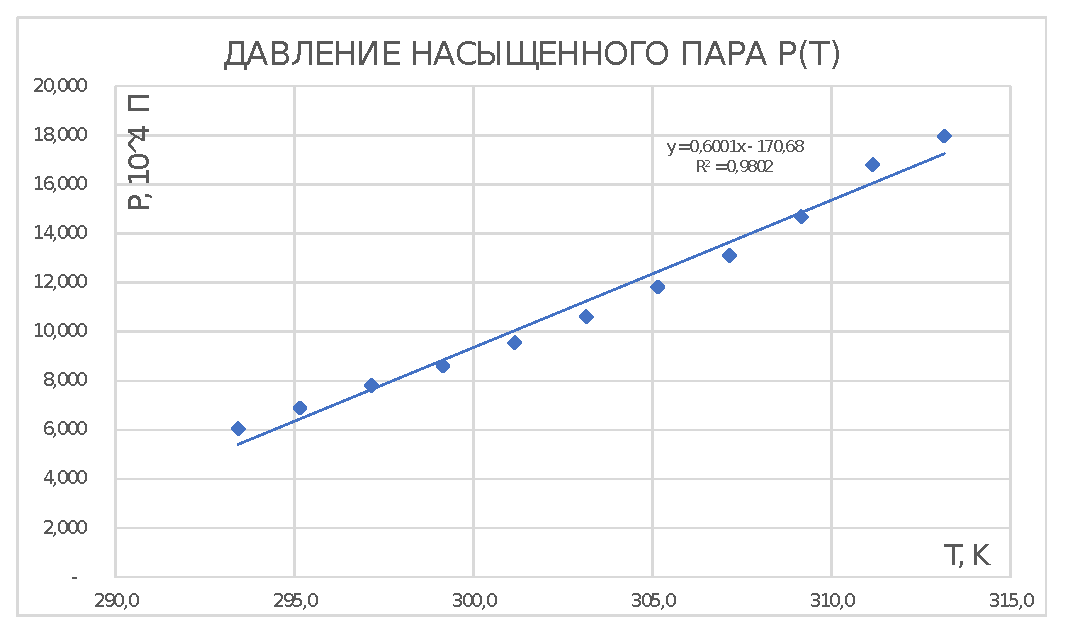
\includegraphics[scale=0.9]{conv1.eps}
\caption{График зависимости P(T) основнанный на измерениях \textit{Таблицы 1-2}}
\end{figure}

\begin{figure}[h]
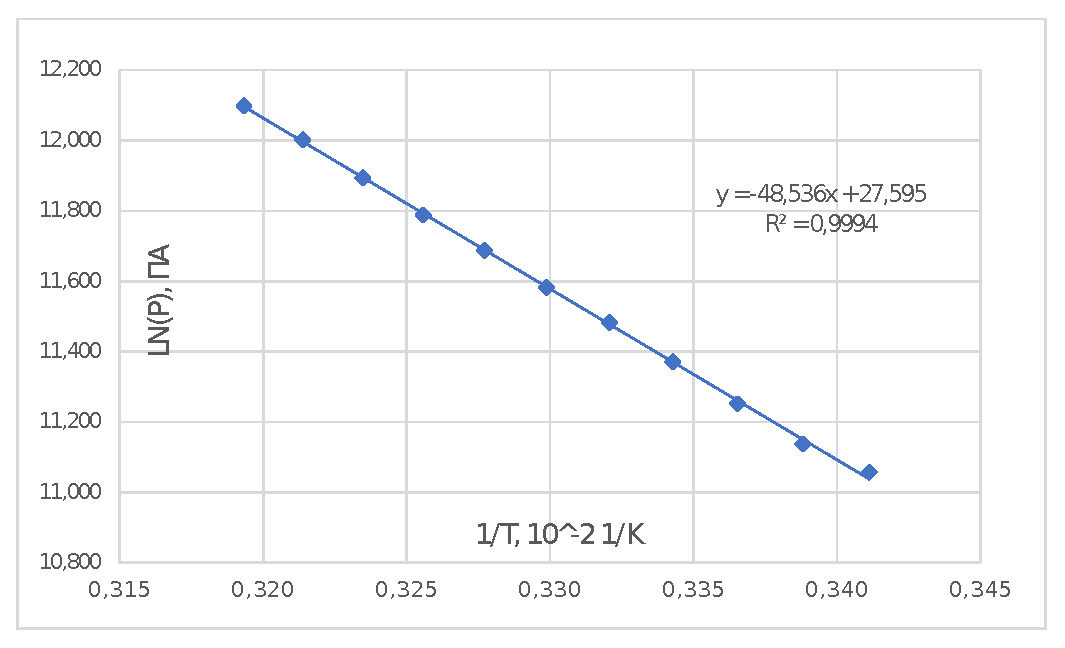
\includegraphics[scale=1]{conv2.eps}
\caption{График зависимости $lnP(1/T)$ основнанный на измерениях \textit{Таблицы 1-2}. Который используется нами для поиска L - теплоты испарения жидкости СПОСОБОМ 2}
\end{figure}


\item
С помощью данных на графике рассчитаем значение L. \\
\textbf{Для первого графика}(\textit{Способ 1}):
\[ L_1 = \dfrac{1}{n} \sum_{i=1}^{n}\dfrac{RT_i^2}{P_i}\Bigl(\dfrac{dP}{dT}\Bigr)_i\]
где $\Bigl(\frac {dP}{dT}\Bigr) \approx 581,3\cdot10^{-3}$. Получаем $L_1 \approx  44390$ Дж/моль. Погрешность измерений:

\[\dfrac{\sigma_{L_1}}{L_1} = \sqrt{2\Bigl(\dfrac{\sigma_T}{T}\Bigr)^2 + \Bigl(\dfrac{\sigma_P}{P}\Bigr)^2 + \Bigl(\dfrac{\sigma_{\frac{dP}{dT}}}{\frac{dP}{dT}}\Bigr)^2}\]

$\dfrac{\sigma_{L_1}}{L_1} = \sqrt{2(\dfrac{4,9}{302,5})^2 + (\dfrac{2716,7}{9786,8})^2 + (\dfrac{159,9}{521,3})^2} \approx 7$

\newpage

\textbf{Для второго графика}(\textit{Способ 2}):
\[L_2 = -R\dfrac{d(\ln P)}{d(1/T)}\]
Получим $L_2 \approx 41294$ Дж/моль. Погрешность измерений:
\[ \sigma_L \approx \frac{R}{\sqrt{n}}\sqrt{\dfrac{<(\ln P)^2> - <\ln P>^2}{<\dfrac{1}{T^2}> - <\dfrac{1}{T}>^2} - k^2}\]

\[\sigma_L \approx  \frac{8,31}{\sqrt{11}}\sqrt{4866^2 - \dfrac{ 134,152 - 134,040}{2\cdot 10^{-7} }  } \approx 475,1\]
\\[2ex]

\subsection*{\Large{Результаты:}}
Занесем полученные результаты в таблицу:

\begin{table}[h!]
\begin{center}
\begin{tabular}{|c|c|c|c|c|c|} 
\hline1
\textbf{$L_1$ Дж/моль} &\textbf{ $L_1$, кДж/кг} & \textbf{$\varepsilon_{L_1}$, \%} &  \textbf{$L_2$, Дж/моль} & \textbf{$L_2$, кДж/кг}. & \textbf{$\varepsilon_{L_2}$, \%}  \\
\hline
43620,0 & 946,82 & 7 & 41294,5 & 896,33 & 2 \\
\hline

\end{tabular}
\caption{Результаты измерения удельной теплоты испарения спирта}
\end{center}
\end{table}

\end{enumerate}

\section{Вывод}
\rhead{Вывод}

В ходе эксперимента было установлено, что использование способа расчета с помощью второго графика позволяет добиться значительно меньших погрешностей, чем расчет с помощью первого графика. 
Полученное значение удельной теплоты испарения спирта составляет 946,82 кДж/кг, что не совсем соответствует табличным данным(837 кДж/кг).
Погрешность эксперимента может
быть объяснена недостаточным временем между экспериментальными
точками, так как, возможно, жидкость и пар не успевали прийти в
динамическое равновесие. Также погрешность вызваны пренебрежением
коэффициентами в уравнении Ван-дер-Ваальса.
\end{document}